%
%===============>>  Мецгер Модуль 6 <<=============
%=
\setmodule{6}

%BEGIN_FOLD % ====>>_____ Занятие 1 _____<<====
\begin{class}[number=1]
	\begin{listofex}
		\item 
	\end{listofex}
\end{class}
%END_FOLD

%BEGIN_FOLD % ====>>_ Домашняя работа 1 _<<====
\begin{homework}[number=1]
	\begin{listofex}
		\item 
		\begin{minipage}[t]{\bodywidth}
			На рисунке изображён график функции вида \( f(x)=ax^2+bx+c \), где числа \( a, b, c \) --- целые. Найдите значение \(f(-3)\).
		\end{minipage}
		\hspace{0.02\linewidth}
		\begin{minipage}[t]{\picwidth}
			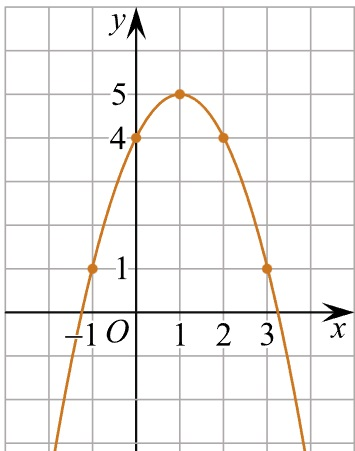
\includegraphics[align=t, width=\linewidth]{../\picpath/MECGERM6H1-1}
		\end{minipage}
		\item 
		\begin{minipage}[t]{\bodywidth}
			На рисунке изображён график функции вида \( f(x)=\dfrac{x^2}{a}+bx+c \), где числа \( a, b, c \) --- целые. Найдите значение \(f(12)\).
		\end{minipage}
		\hspace{0.02\linewidth}
		\begin{minipage}[t]{\picwidth}
			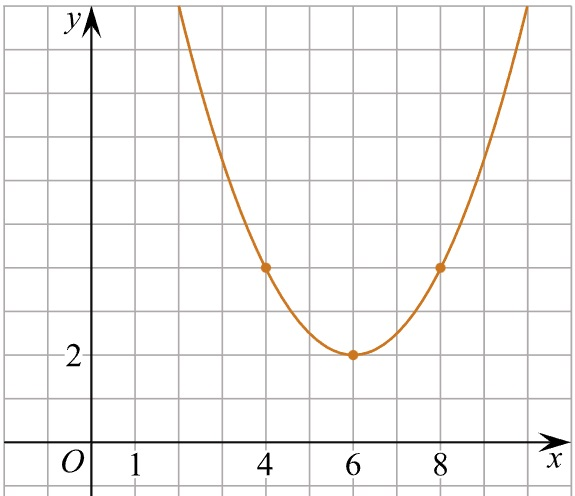
\includegraphics[align=t, width=\linewidth]{../\picpath/MECGERM6H1-2}
		\end{minipage}
		\item
		\begin{minipage}[t]{\bodywidth}
			На рисунке изображён график функции вида \( f(x)=\dfrac{a}{x+b}+c \), где числа \( a, b, c \) --- целые. Найдите значение \(f(9)\).
		\end{minipage}
		\hspace{0.02\linewidth}
		\begin{minipage}[t]{\picwidth}
			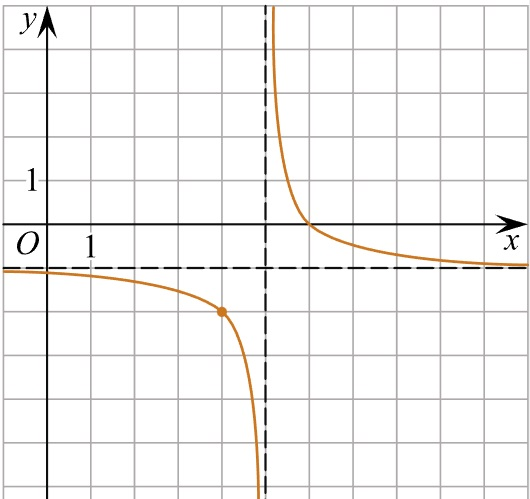
\includegraphics[align=t, width=\linewidth]{../\picpath/MECGERM6H1-3}
		\end{minipage}
		\item
		\begin{minipage}[t]{\bodywidth}
			На рисунке изображён график функции вида \( f(x)=\dfrac{k}{x}+a \). Найдите значение \(f(-12)\).
		\end{minipage}
		\hspace{0.02\linewidth}
		\begin{minipage}[t]{\picwidth}
			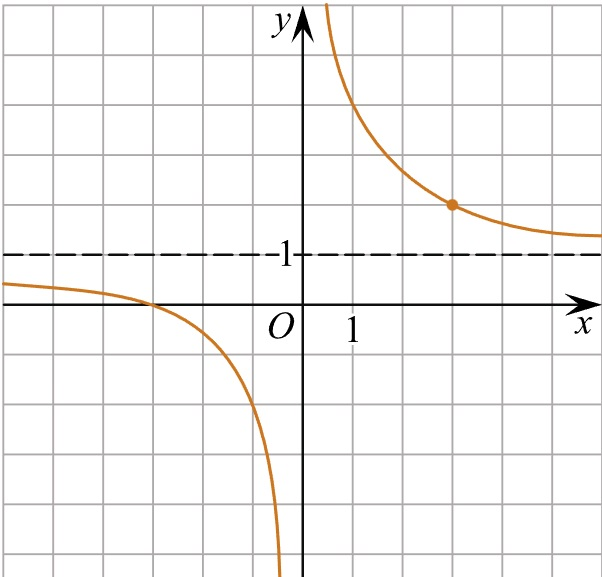
\includegraphics[align=t, width=\linewidth]{../\picpath/G101M4C4-7}
		\end{minipage}
		\item Найдите значение выражения: \( 8\sin{\dfrac{5\pi}{12}}\cdot\cos{\dfrac{5\pi}{12}} \)
		\item Найдите значение выражения: \( \dfrac{34\sin{406\degree}}{\sin{46\degree}} \)
		\item Найдите значение выражения: \( \dfrac{3^{6,5}}{9^{2,25}} \)
		\item Найдите значение выражения: \( 4^8 \cdot 11^{10} : 44^8 \)
		\item Найдите значение выражения: \( \dfrac{(\sqrt{13}+\sqrt{7})^2}{10+\sqrt{91}} \)
		\item Найдите корень уравнения: \( \sqrt{-4-5x}=4 \)
		\item Решите уравнение: \( \sin{\dfrac{\pi x}{3}}=0,5 \). В ответе напишите наименьший положительный корень.
	\end{listofex}
\end{homework}
%END_FOLD

%BEGIN_FOLD % ====>>_____ Занятие 2 _____<<====
\begin{class}[number=2]
	\begin{listofex}
		\item Занятие 2
	\end{listofex}
\end{class}
%END_FOLD

%BEGIN_FOLD % ====>>_ Домашняя работа 2 _<<====
\begin{homework}[number=2]
	\begin{listofex}
		\item
		\begin{minipage}[t]{0.7\linewidth}
			На рисунке изображён график функции вида \[f(x)=ax+|bx+c|+d\], где числа \(a, b, c, d\) --- целые. Найдите корень уравнения \(ax+d=10\).
		\end{minipage}
		\begin{minipage}[t]{0.25\linewidth}
			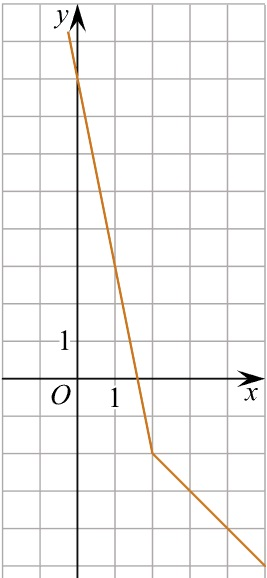
\includegraphics[align=t, width=\textwidth]{../\picpath/G111M4C5-4.jpg}
		\end{minipage}
		\item
		\begin{minipage}[t]{\bodywidth}
			На рисунке изображён график функции вида \[ f(x)=ax-|bx+c|+d, \] где числа \(a, b, c, d\) --- целые. Найдите корень уравнения \(ax+d=0\).
		\end{minipage}
		\hspace{0.02\linewidth}
		\begin{minipage}[t]{\picwidth}
			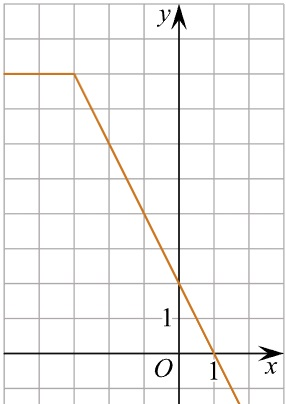
\includegraphics[align=t, width=\linewidth]{../\picpath/K-L8.jpg}
		\end{minipage}
	\end{listofex}
\end{homework}
%END_FOLD

%BEGIN_FOLD % ====>>_____ Занятие 3 _____<<====
\begin{class}[number=3]
	\begin{listofex}
		\item Занятие 3
	\end{listofex}
\end{class}
%END_FOLD

%BEGIN_FOLD % ====>>_ Домашняя работа 3 _<<====
\begin{homework}[number=3]
	\begin{listofex}
		\item
		\begin{minipage}[t]{\bodywidth}
			На рисунке изображён график функции \[ f(x)=a \cos{x}+b \] Найдите \(a\).
		\end{minipage}
		\hspace{0.02\linewidth}
		\begin{minipage}[t]{\picwidth}
			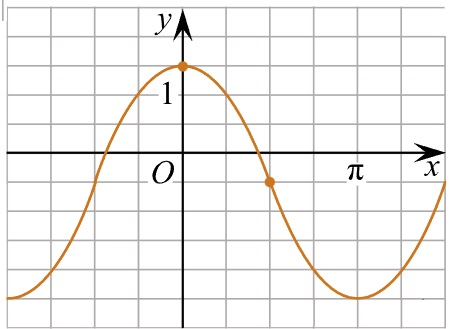
\includegraphics[align=t, width=\linewidth]{../\picpath/MECGERM6H3-1.jpg}
		\end{minipage}
		\item
		\begin{minipage}[t]{\bodywidth}
			На рисунке изображён график функции \[ f(x)=a \tg{x}+b \] Найдите \(a\).
		\end{minipage}
		\hspace{0.02\linewidth}
		\begin{minipage}[t]{\picwidth}
			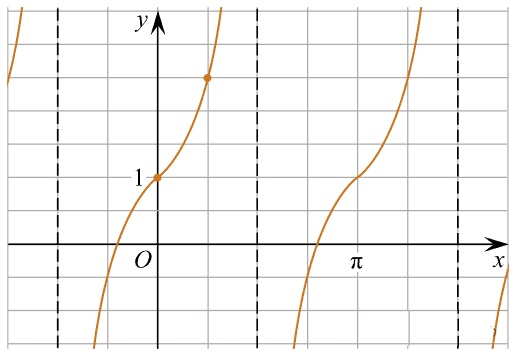
\includegraphics[align=t, width=\linewidth]{../\picpath/MECGERM6H3-2.jpg}
		\end{minipage}
		\item
		\begin{minipage}[t]{\bodywidth}
			На рисунке изображён график функции \[ f(x)=a^x+b \] Найдите значение \(x\), при котором \( f(x)=29 \).
		\end{minipage}
		\hspace{0.02\linewidth}
		\begin{minipage}[t]{\picwidth}
			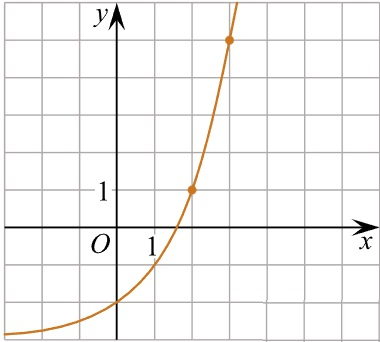
\includegraphics[align=t, width=\linewidth]{../\picpath/MECGERM6H3-3.jpg}
		\end{minipage}
		\item Найдите значение выражения \( \dfrac{7\sqrt{x}-5}{\sqrt{x}}+\dfrac{5\sqrt{x}}{x}+3x-4 \) при \( x=3 \).
		\item Найдите значение выражения \( \dfrac{6}{\cos^2{23\degree}+\cos^2{113\degree}} \).
		\item Найдите значение выражения \( 2\sqrt{2}\cos^2{\dfrac{3\pi}{8}}-\sqrt{2} \).
	\end{listofex}
\end{homework}
%END_FOLD

%BEGIN_FOLD % ====>>_____ Занятие 4 _____<<====
\begin{class}[number=4]
	\begin{listofex}
		\item Пусто
	\end{listofex}
\end{class}
%END_FOLD


%BEGIN_FOLD % ====>>_ Проверочная работа _<<====
\begin{exam}
	\begin{listofex}
		\item Проверочная
	\end{listofex}
\end{exam}
%END_FOLD